\chapter{Color Coding}
\label{cap 2}
In questo capitolo verr\`a descritta la tecnica del Color Coding utilizzata in questa tesi.

La tecnica fu introdotta nel 1995 da Alon, Yuster e Zwick \cite{alon1995color}.
In generale, dati due grafi $G$ ed $ H $ , il problema di individuare un sottografo indotto di $ G $ isomorfo ad $ H $ \`e un problema $ NP $-completo, ma pu\`o essere risolto in tempo polinomiale tramite un algoritmo randomizzato per classi particolari di grafi $ H $, usando la tecnica del color coding.

Il primo algoritmo che Alon e i suoi colleghi descrissero in \cite{alon1995color} , per\`o, risolve tale problema quando $ H $ \`e un cammino o un albero con treewidth costante limitandosi, inoltre, alla sola ricerca senza farne un conteggio del numero delle occorrenze totali.
 
In questo capitolo, si presenta un'estensione dell'algoritmo descritto da Alon \cite{alon1995color,bressan2018motif} che per effettuare un conteggio delle occorrenze di tutti i treelet all'interno del grafo.\\




\section{Algoritmo}
\label{section1}

Dati in input un grafo $ G=(V,E) $ ed un intero positivo $ k $, per prima cosa il color coding assegna indipendentemente ed uniformemente a caso un \emph{colore}  $c_v \in [k] = \{1,....,k\} $ ad ogni nodo  $ v\in V $ di $ G $.
Dato un sottografo $H$ di $G$, diremo che $H$ è \emph{ben colorato} se ogni nodo $v$ di $H$ ha un colore $c_v$ distinto.

Il cuore dell'algoritmo consiste nel conteggiare il numero di occorrenze (non necessariament indotte) di alberi ben-colorati di $k$-nodi in $ G $.
%, chiamati $ k-treelet $, in cui ogni vertice dell'occorrenza ha un colore distinto.
Questo viene fatto in maniera efficiente mediante programmazione dinamica, una tecnica che risolve dei sottoproblemi del problema di interesse, procedendo dai problemi ``pi\`u piccoli'' verso quelli ``pi\`u grandi'' e ricostruendo le relative soluzioni in funzione delle soluzioni già calcolate per i problemi precedentemente risolti, fino a risolvere il problema originario.

Nel seguito deneoteremo con $ T_C $ un \emph{treelet colorato}, ovvero una coppia $ (T,C) $ dove $ T $ un albero radicato e $ C \subseteq \{1,\dots,k\}$.
Per ogni nodo $ v \in V $ e per ogni treelet colorato $ T_C $, con $ k $ nodi, si vuole calcolare il numero $ c(T_C , v) $ di occorrenze (non indotte) di $ T_C $  in $ G $ che sono radicate in $v$.\\
Inizialmente per ogni nodo $ v $ si inizializza $ c(T_C , v) = 1 $, dove $T$ \`e il treelet di $1$ nodo e $ C = \{c_v\}$.
Dopodichè, per ogni $ h = 2,\dots,k $,  si considera ogni possibile albero radicato $T$ di dimensione $ h $, ogni possibile insieme di colori $ C \subseteq [k] $ con $ |C| = h $, ed ogni nodo $v \in V$.
%Il numero $ c(T_C,v) $ di occorrenze dei treelet (non indotti) radicati in $ v $ isomorfi a $ T $ e i cui colori giacciono nell'insieme $ C $.\\
L'albero $T_C$ viene \emph{decomposto} in due alberi $T'$ e $T''$
come segue: $ T'' $ \`e il sottoalbero radicato in uno dei figli della radice $ v $ di $ T $ e $ T' $ \`e il sottoalbero di $ T $ radicato in $ v $ contenente $ |T| - |T''| $ nodi.
TODO Non va bene: ci sono tanti sottoalberi di $T$ che contengono $ |T| - |T''| $ nodi. Quale prendi?

Ne segue che, per un'opportuna partizione dei colori $C$ in due insiemi $C$ e $C'$, ogni occorrenza di $T_C$ in $G$ implica l'esistenza due due occorrenze distinte $T'_{C'} = (T', C')$ e $T''_{C''} = (T'', C'')$  in $G$ radicate, rispettivamente nei nodi $v$ e $u$.
Viceversa, ogni coppia di occorrenze $T'_{C'}$ e $T''_{C''}$ radicate, rispettivamente, in $v$ e $u$ induce un'occorrenza (non necessariamente distinta) di $T_C$ radicata in $v$.
In particolare è facile ossevare che, chiamato $\beta_T$ è il numero di sottoalberi di $T$ radicati in un figlio di $r$ isomorfi a $T''$, esistono esattamente $\beta_T$ coppie di occorrenze $T'_{C'}$ e $T''_{C''}$ che inducono $T_C$. 

Dalla discussione seguente segue che, per calcolare $ c(T_C,v)$ è sufficiente considerare tutti treelet colorati radicati in $ v $ isomorfi a $ T'_{C'} $ e tutti i  treelet radicati in un vicino $ u $ di $v$ isomorfi a $ T''_{C''} $, tali che $ C',C'' \subseteq [k] $ con  $C' \cup C'' = C$ e $C' \cap C' = \emptyset$. %$ |C'|=i $ e $ |C''| = k-i $ \\ TODO NO!!!  :(
Sia per $ T' $ che per $ T'' $ \`e noto il numero di occorrenze $ c(T'_{C'},v) $ e $ c(T_{C''},u) $ in $ G $, poich\`e $|T'|, |T''| \le h-1$. Pertanto:

\begin{equation}\label{conta}
	c(T_c,v)=\frac{1}{\beta_T}\sum_{(u,v)\in E} \;\; \sum_{\substack{C', C'' \subset C : |C'| = |T'| \\C' \cup C'' = C  \\ C' \cap C'' = \emptyset}}c(T'_{C'},v)\cdot c(T''_{C''},u).
\end{equation}

 La correttezza e la complessit\`a di questo algoritmo, non sono trattate in questa tesi, ma vengono dimostrate da Alon in \cite{alon1995color}.\\
 Si pu\`o vedere l'algoritmo formalmente  descritto in Algoritmo \ref{algoritmo}.


\begin{algorithm}[H]
	\caption{TODO}
	\label{algoritmo}
	\SetAlgoLined
 	\textbf{input} : Grafo $ G =(V,E) $, dimensione del treelet $ k $ ,insieme [$ k $] di colori\;	
 		\For{$ v  \in V$}{
 			Sia $c_v $ un colore scelto uniformemente a caso in [$ k $]\;
 			Sia $T$ il treelet contenente un solo nodo\;
 			$T_C = (T, \{c_v\})$\; 
 			$ c(T_C, v) = 1 $\;
 		}	
 			\For{$ h = 2$ to $ k $}{
 				\For{$ v \in V $}{
 					\ForEach{$ T : |T| = h $}{
 							Suddivido $ T $ in due alberi $ T'$	 e  $ T'' $ come descritto in precedenza. %TODO In precedenza dove? Metti il riferimento alla sezione
 						\( 	c(T_c,v)=\frac{1}{\beta_T}\sum_{(u,v)\in E} \;\; \sum_{\substack{C', C'' \subset C : |C'| = |T'| \\C' \cup C'' = C  \\ C' \cap C'' = \emptyset}}c(T'_{C'},v)\cdot c(T''_{C''},u) \)	
 					}
 				}
 			}
 			
\end{algorithm}\mbox{}\\

Come si pu\'o notare, per calcolare le occorrenze di un albero $ T_C $ nell'algoritmo si sfrutta un approccio top-down, ossia, a partire dall'albero $ T_C $, si identificano i due alberi $ T' $ e $ T'' $ in cui pu\`o essere scomposto, si considerano tutte le partizioni di $ C',C'' \subset C $ e in seguito si procede al calcolo di $ c(T_C,v) $ come indicato in \eqref{conta}.

In questa tesi, cos\'i come in \cite{bressan2019motivo}, si \`e sfruttato un approccio bottom-up. Infatti, per ogni nodo $ v \in V $ di $ G $ e per ogni nodo $ u \in V$ con $ (u,v)\in E $ si prendono tutte le coppie possibili di treelet colorati radicati  in $ v $ e $ u $, rispettivamente $ T'_{C'} $ e $ T''_{C''} $, e si verifica se esiste un albero $T_C$ radicato in $v$ per cui la coppia  $ T'$ e $ T''$ rappresenta una decomposizione ammissibile e tale che $C'$ e $C''$ sono una partizione di $C$.
Sar\`a, pertanto, necessario che dati due alberi $ T' $ e $ T'' $ la sia tale che: $ |T'|,|T''|>0 $ e che $ |T'| + |T''| = k $. %TODO La notazione |T| è già usata in precedenza, pertanto deve essere definita prima (e non qui)


% TODO tutto il pezzo sotto sembra magico. Perchè "viene supposto"? Qual è la ragione? Perchè funziona? Tra l'altro la regola usata è sbagliata... Rivedila bene

%Inoltre viene supposto di voler ottenere solo i $ k $-treelet $ T $ in cui i sottoalberi radicati nella radice $ r $ abbiano un ordinamento non crescente.
%Perci\`o se la cardinalit\`a di $ T'' $ supera la cardinalit\`a del sottoalbero radicato nell'ultimo figlio della radice di $ |T'| $, non \`e possibile compiere l'unione tra i due.

Si noti che i conteggi del numero di occorrenze di ogni $ k $-treelet colorato raggiungibile da ogni nodo $ v\in V $ di $ G $, %TODO cosa è un treelet colorato *raggiungibile* da un nodo? 
sono svolti e salvati in maniera separata.
Lo scopo di questa tesi per\`o \'e quello di stimare, per ogni $k$-treelet $T^*$, il numero $N(T^*)$ di  sottografi (non necessariamente indotti) isomorfi $T^*$ nel grafo $ G $.
A tal proposito si noti che ogni occorrenza $O$ di un generico $k$-treelet $T$ in $G$ è responsabile dell'incremento di $1$ di esattamente $k$ contatori $c(T_C, v)$. In particolare tali contatori si riferiscono ai nodi $v$ di $O$ e agli alberi $T_C = (T,C)$ per cui $C = \{1, \dots, k\} $ e $T$ è ottenuto radicando $T$ nel nodo corrisponte a $v$.

Sia $\mathcal{T}$ l'insieme di tutti gli alberi isomorfi a $T$ e $\widetilde{N}(T)$ il numero di occorrenze ben colorate di $T$ in $G$. Dalla discussione precedente segue che:
$\widetilde{N}(T) = \frac{1}{k}\sum_{T \in \mathcal{T}} \sum_{v \in V} c( T_C, v)$ dove $T_C = (T, \{1,\dots, k\})$. 

Inoltre, poich\`e ogni occorrenza di un $k$-treelet $T$ in $G$ è ben colorata con probabilità $\frac{k!}{k^k}$, uno stimatore unbiased del numero di $N(T^*)$ è $\frac{k^k}{k!} \cdot \widetilde{N}(T)$, cioè
$\mathbb{E}\left[\frac{k^k}{k!} \cdot \widetilde{N}(T)\right] = N(T^*)$.


%TODO
%Per favore rivedi il resto di questa sezione. Spiega il trucco di contare  c(T_C, v) solo nei nodi v per cui c_v = 0 e come questo cambia \widetilde{N}(T).
%Spiega BENE la questione delle classi di equivalenza e del rappresentante.
%Adesso dici che serve per "evitare di conteggiare gli alberi un numero di volte superiori a quelle effettive" ma questo è falso. 





 per ogni $k$-treelet $T_C = (T, \{1, \dots, k\})$, 
è neccessario aggregare i conteggi $c(T_C, v)$ memorizzati nei vari nodi $v \in V(G)$ in modo da ottnere il numero $N(T)$ occorrenze complessivo per ogni possibile $ k $-trelet.

%NO!! Questo non serve a evitare di conteggiare gli alberi troppe volte....
Per evitare di conteggiare gli alberi un numero di volte superiori a quelle effettive, si considerano le classi di equivalenza dell'insieme degli alberi di $ k $ nodi, in cui gli alberi di ogni classe sono isomorfi tra loro.
Per ogni classe di equivalenza viene scelto un opportuno rappresentante , $ \tau(T) $, che aggrega tutti i conteggi delle occorrenze relativi alla classe che rappresenta. \\
 Dati due alberi $ T' = (V',E')$ e $ T''=(G'',E'') $ si dicono isomorfi se esiste una funzione bijettiva $ f : V' \rightarrow V'' $ tale che $ (u,v)\in E' $ se e solo se $ (f(u),f(v)) \in E' $.\\
Perci\`o se due alberi sono isomorfi verranno raggruppati nella stessa classe di equivalenza e le loro occorrenze saranno sommate.
Cos\`i facendo otterremo i conteggi effettivi di tutti i $ k $-treelet colorati trovati in $ G $ e il numero di volte che occorrono nel grafo.
Poich\`e quello che interessa \`e il conteggio di tutti i $ k $-treelet in un grafo, sar\`a necessario tener conto che per ogni nodo colorato $ v\in V $ ogni albero viene conteggiato un numero $ k $ superiore di volte, una volta in pi\`u per ogni colore differente di radicamento, quindi per calcolare il numero corretto sar\`a sufficiente dividere il numero dei conteggi delle occorrenze per $ k $.
Inoltre, poich\`e il numero delle occorrenze di un treelet colorato in un grafo subisce un fattore di normalizzazione pari a $ \frac{k!}{k^k} $.
Per calcolare il numero di occorrenze di tutti i $ k $-treelet colorati sar\`a sufficiente fare quanto segue.
Per ogni albero $ T $ tale che $ T_C $ \`e l'albero colorato in $ C=\{1,\dots, k\} $, si ha che $ N(T) $, il conteggio delle occorrenze di $ T $ in $ G $ \`e pari a:
\[N(T) = \frac{1}{k} \cdot \frac{k^k}{k!} \cdot \sum_{v\in V} c(T_C,v) \]


\section{Dettagli implementativi. Rappresentazione compatta dei treelet colorati e rispettivi conteggi}
\label{section 2}
In questa sezione vengono descritte le strutture dati usate per implementare l'algoritmo in Java.
Gli oggetti principali che vengono manipolati sono i treelet colorati e le occorrenze associate.

Ogni treelet colorato $ T_C = (T,C) $ ha una rappresentazione unica nella quale sono memorizzate la topologia di $ T $, i colori in $ C $ ed informazioni aggiuntive per facilitare la minipolazione di $T_C$.
Tale rappresentazione richiede al pi\`u 58 bit e pu\`o pertanto essere memorizzata usando degli interi a 64 bit, un tipo di dati nativo in Java, nelle pi\`u comuni architetture moderne.
I bit sono numerati da 0 a 63 e ordinati dal bit meno significativo a quello pi\`u significativo.\\
Sono cos\'i suddivisi:
\begin{itemize}
	\item i bit da 0-3 contengono il numero di nodi di $ T $ a meno della radice.
	\item i bit da 4-7 contengono la dimensione del sottoalbero radicato nell'ultimo figlio della radice di $ T $.
	\item i bit da 8-11 vengono usati per memorizzare il valore di $ \beta_T $ associato a $ T $.
	\item i bit da 12-27 sono usati per indicare i colori in $ C $.
	\item i bit da 28-58 sono usati per codificare la struttura del treelet, come descritto di seguito.
	\item gli ultimi 5 bit sono lasciati a zero.
\end{itemize}\mbox{}

Per codificare la struttura dell'albero si procede a partire da una visita in profondit\`a (DFS) su $ T $.\\
In questo caso la visita avviene partendo dalla radice $ r $ di $ T $ e attraversando tutti gli archi. Al termine ogni arco sar\`a stato attraversato esattamente 2 volte, in direzioni opposte. \\
Sia $h=|T|$ e sia $e_i$, con $i = 1, 2, \dots, 2(h-1)$, l'$i$-esimo arco attraversato dalla visita. 
L'$i$-esimo bit della codifica \`e $0$ se $e_i$ \`e attraversato in direzione di $r$ in $T$ e $1$ in caso contrario.\\
 In Figura \ref{figura} si pu\`o vedere un esempio di tale codifica.

\begin{figure}[htbp]
	\centering
	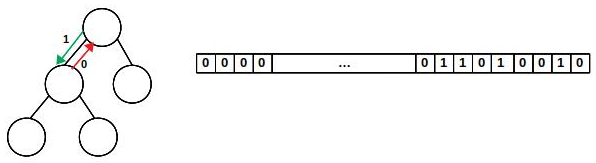
\includegraphics[width=11cm]{capitolo2/grafo3}
	\caption{Un treelet radicato e la codifica della sua struttura}
	\label{figura}
\end{figure}

Per un qualunque $ k \le 16 $ questa codifica richiede al massimo 30 bit.
L'ordinamento lessicografico sulla struttura definisce anche implicitamente un'ordinamento totale sui treelet. Questo ordinamento \`e anche una regola decisiva per la visita DFS: i figli di un nodo vengono visitati nell'ordine indotto dai sottoalberi radicati in essi.
Ci\`o implica che ogni treelet $ T $ ha una codifica unica ed ogni codifica valida corrisponde ad un solo treelet. Inoltre, in questo modo \`e possibile implementare rapidamente l'operazione di unione.\\\\
La codifica dei treelet supporta le seguenti operazioni :
\begin{itemize}
	\item $ \textbf{singleton} $ (c) : permette di inizializzare un treelet di un solo nodo con il rispettivo colore $ c \in \{1, \dots, k\} $
	\item $ \textbf{merge} $ ($ T'_{C'} $,$ T''_{C''} $) : fa l'unione di due alberi $ T' $ e $ T'' $ e se possibile crea un nuovo albero $ T $ che avr\`a come struttura la concatenazione delle strutture di $ T' $ e $ T'' $ (a meno della radice).
	La dimensione, a meno della radice, sar\`a data dalla somma delle dimensioni di $ T' $ e $ T'' $ pi\'u 1.
	I colori di $ T $, sono il risultato dell'unione dei colori di $ T' $ e $ T'' $.
	$ \beta_T $ sar\`a, inizialmente, pari al valore $ \beta_{T'} $ corrispondente a $ T' $ e se la struttura del sottoalbero radicato nell'ultimo figlio di $ T' $ \`e uguale alla struttura di $ T'' $ viene eventualmente incrementato di 1.\\
 	 Per finire, la dimensione del sottoalbero pi\`u piccolo radicato in $ T $ sar\`a esattamente la dimensione di $ T'' $, a meno della radice, pi\`u 1 .
	\item $\textbf{normalization\_factor}$ ($ T_C $): restituisce la costante di normalizzazione $ \beta_T $ associata a $ T_C $.
	    
\end{itemize}
\begin{figure}[htbp]
	\centering
	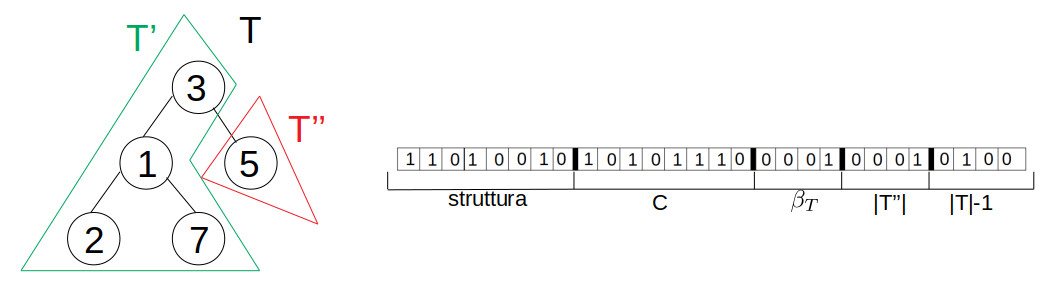
\includegraphics[width=11cm]{capitolo2/grafo5}
	\caption{un treelet colorato $ T_C =(T,C) $ e la sua codifica, mostrata per semplicit\`a solo su 8+8+4+4+4=28 bit}
	\label{figura1}
\end{figure}
 In Figura \ref{figura1} \`e mostrato un esempio di treelet colorato e della sua codifica\\\\
Nell'implementazione i treelet individuati da ogni nodo e i rispettivi conteggi vengono salvati all'interno di una tabella indicizzata, rappresentata mediante strutture annidate di $ ArrayList $.\\
Inizialmente, come nell'algoritmo \ref{algoritmo}, i treelet e i conteggi sono stati valutati su ogni nodo $ v \in V $ di $ G $ scorrendo tutti gli archi $ E $, quello che si ha, perc\`o \`e una tabella con $ k $ entrate indicizzate da $ 1 $ a $ k $ ed associate al numero di vertici dei treelet.\\ 
L'$ i $-esima entrata della tabella, con $ 1\le i \le k $ generico, a sua volta, \`e un $ ArrayList $, con una dimensione fissata, che varia a secondo della cardinalit\`a di $ V $, cos\`i che ad ogni entrata \`e associato un vertice $ v\in V $ di $ G $.\\
Per ognuna delle $ |V| $ entrate, viene creato un $ ArrayList $ contenente tutti i treelet colorati di dimensione $ i $ raggiungibili dai differenti nodi in $ V $, insieme al relativo numero di occorrenze.\\
All'interno di quest'ultima lista i treelet sono ordinati in ordine non descrescente.

Per permettere una costruzione pi\`u rapida della tabella, nell'implentazione \`e utilizzato il $ Multithreading $, cio\`e vengono utilizzati pi\`u thread che lavorano in parallelo.
Un thread \`e un flusso di esecuzione indipendente all'interno di un processo.
Il numero di thread utilizzato nell'implementazione \`e dipendente dal numero di processori presenti nella macchina.




	
